\section{Background}\label{sec:background}
%
\begin{figure}[ht]
    \centering
    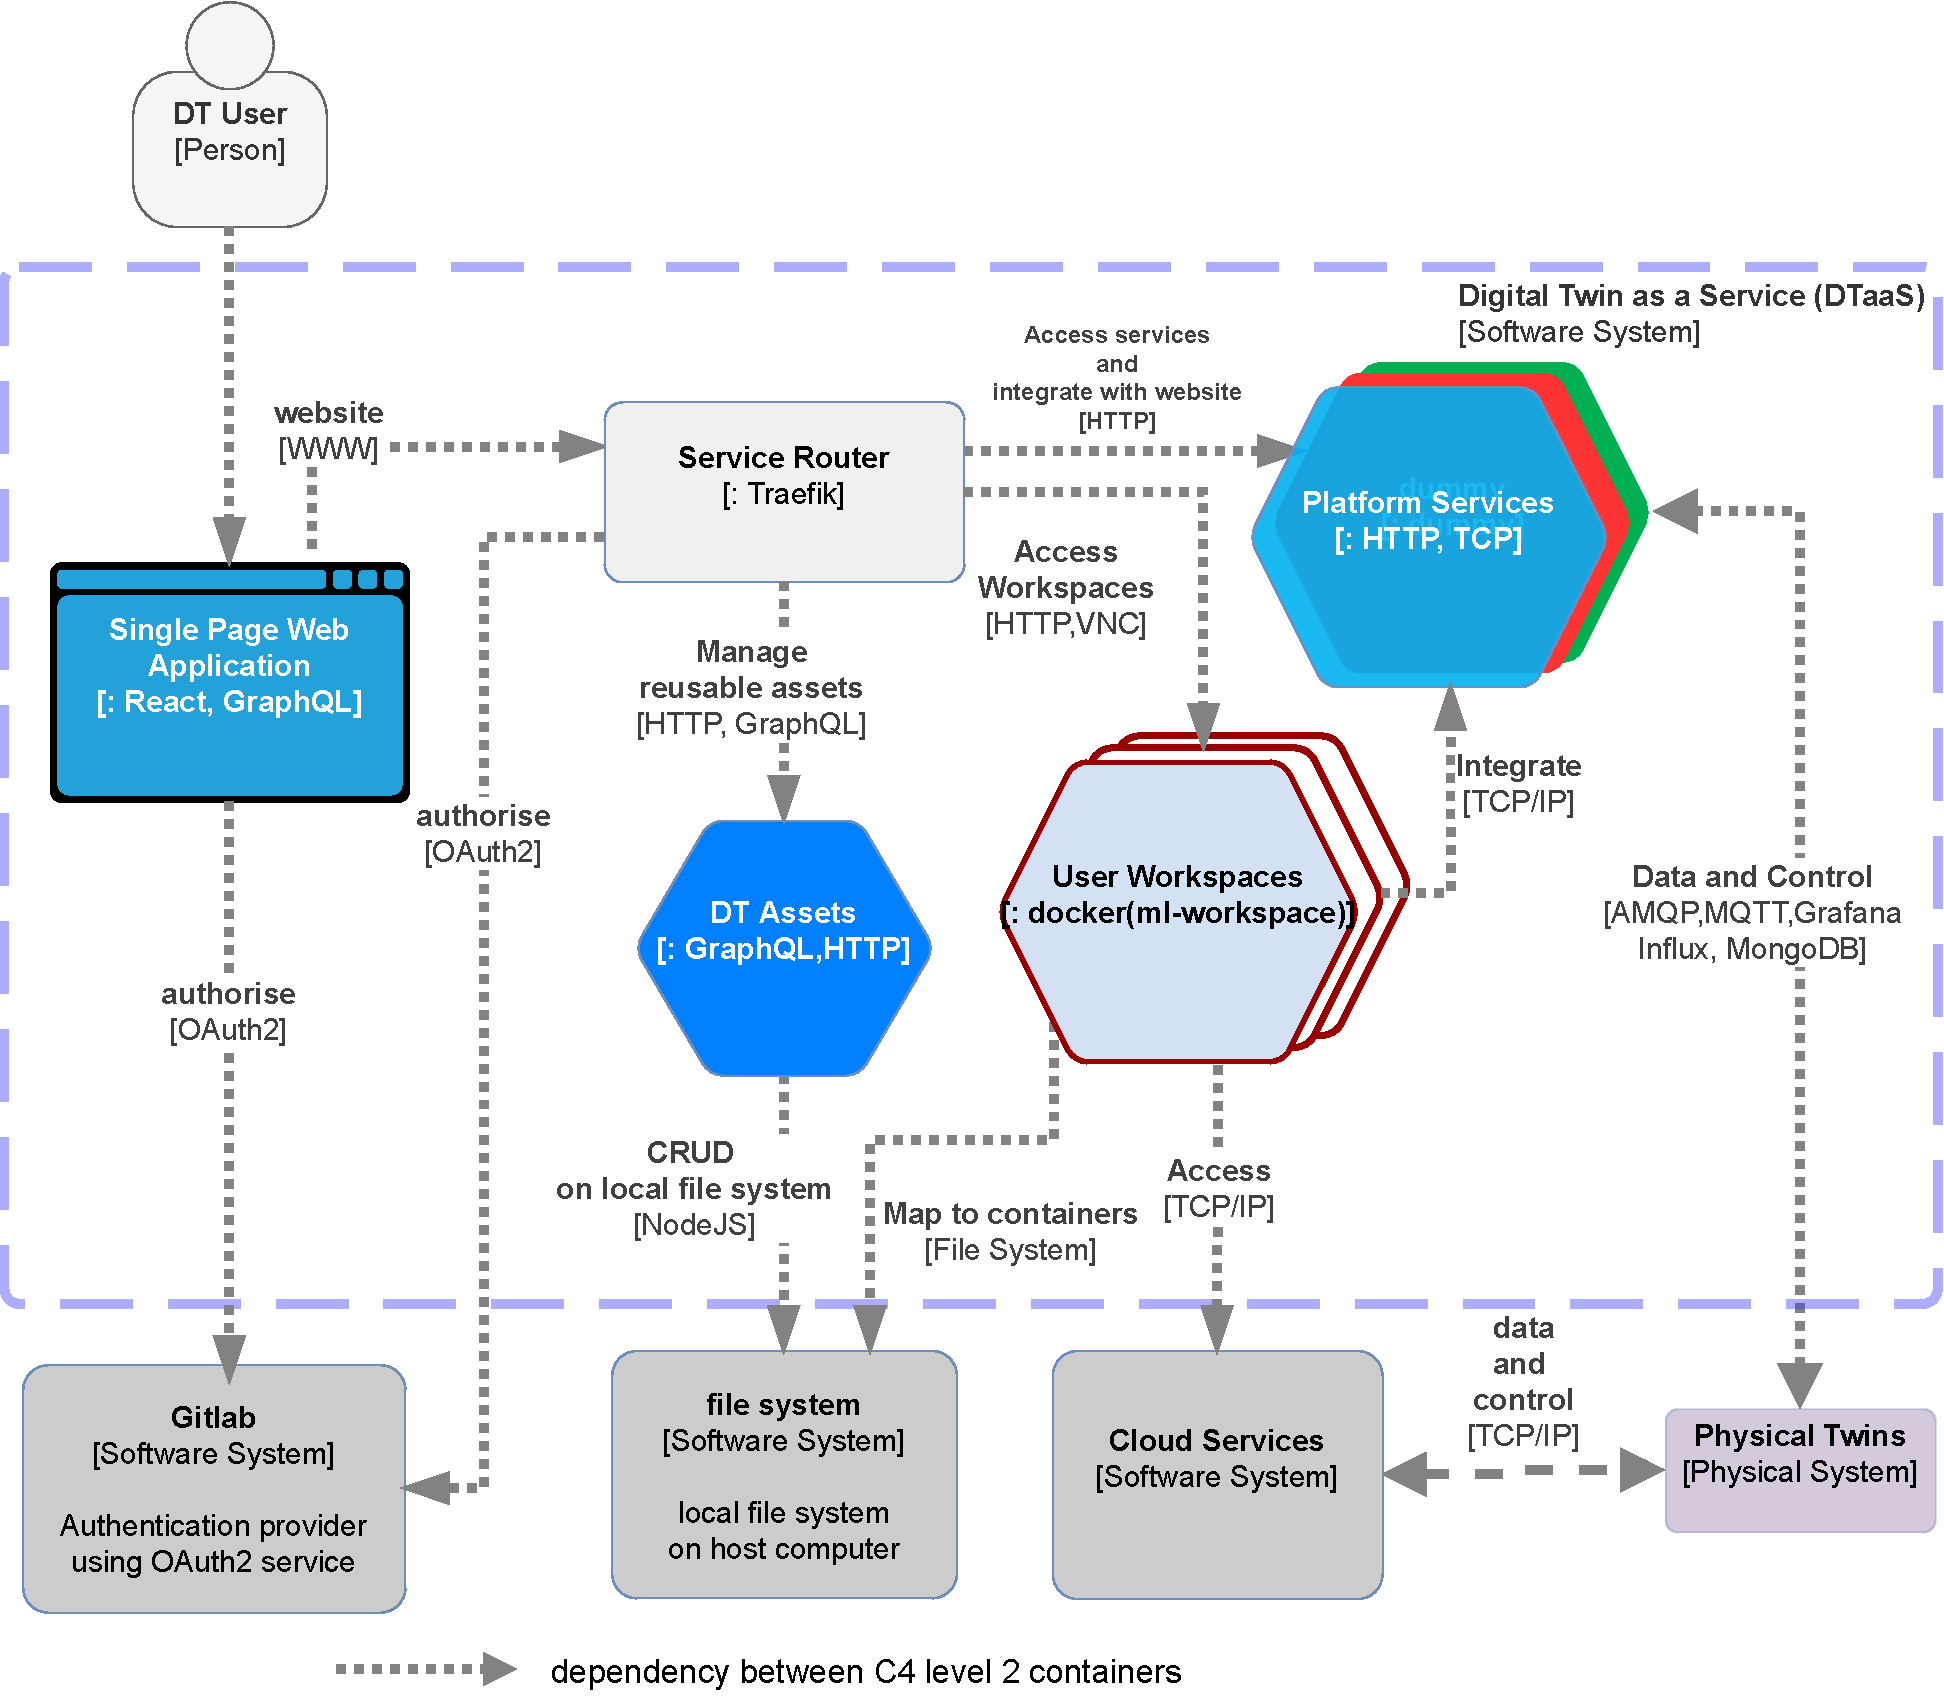
\includegraphics[width=0.9\textwidth]{images/DTaaS-architecture.pdf}
    \caption{Software architecture of the DTaaS software platform. This diagram follows the conventions of the C4 model.}
    \label{fig:dtaas-architecture}
\end{figure}%
%
\subsection{Digital Twins as a Service}
The DTaaS platform is a collaborative platform to build, use, and share DTs. \cref{fig:dtaas-architecture} shows the software architecture of DTaaS. It is a microservices-based architecture with dedicated software containers\footnote{Container is a software component at level-2 of the C4 model.} for DT assets, user workspaces, platform services, a front-end website, and service router.

The separation of concerns is a well-established software engineering principle.
Use of it in the context of DTs is likely to yield significant benefits. One of the architectural principles used in the development of DTaaS is to conceive DTs as composed of reusable assets. These reusable assets separate the functionality provided by DTs into their constituent parts, i.e., DT assets.
The data, models~\cite{Zambrano&22}, tools~\cite{qi2021enabling}, services~\cite{budiardjo2021digital,robles2023opentwins} and ready to use DTs~\cite{aziz2023distributed} have been identified as reusable assets of DTs.
The DT Assets software container provides an interface to perform create, reuse, update, and delete operations on DT assets stored within the DTaaS.
% These DT assets can divided into two categories - private and common.
% Private assets are manageable by their owner whereas common assets are manageable by all users. The users can collaborate at the level of DT assets by sharing them as common assets.
%\morten{Commented out part about public/private assets as it is unimportant to tool providers}

All users have private workspaces in which they can build and use DTs.
Within the context of DTaaS, the creation of DT assets is part of the build phase of DTs.
The workflows involved in building DTs are different from using DTs~\cite{Prasad&21a}. Many DT platforms are dedicated to either building or using DTs but not both. In contrast, DTaaS strives to support both workflows.
The user workspaces access DT assets as a regular part of the filesystem.
All workspaces have access to the Internet and WWW thereby enabling the integration of DTs running inside workspaces with external software systems and PTs.

The platform services are the most often used DT services common across DTs and users. The communication, data storage, visualization, monitoring, and alerts are the most frequently used common services~\cite{qi2021enabling}.
All these services are supported in the DTaaS using RabbitMQ and MQTT (communication), InfluxDB and MongoDB (data storage), and Grafana (monitoring and alerts).
Additionally, it is possible to host private services accessible to a selected number of users. These services include the run-time services provided by TeSSLa and NuRV.

% The front-end website acts as the user interface while the service router acts as a gateway to all the software containers. The OAuth2 service of Gitlab is used to provide user authorisation to the DTaaS\simon{Do we need to mention OAuth2?}.
% \morten{No. Outcommented it.}

\subsection{Runtime Verification}

Many approaches to verification focus on offline analysis through the use of systematic testing, theorem proving, or model checkers such nuXmv~\cite{cavada2014nuxmv}, which aim to catch bugs before a system is deployed.
In contrast, runtime verification focuses on augmenting a system with additional monitoring functionality, in order to catch bugs at runtime.
Runtime verification can complement offline formal methods, as a lightweight method of improving the integrity of deployed systems.
As surveyed in~\cite{sanchez2019advancedrvsurvey}, runtime verification can also be applied to classes of systems that challenge leading offline methods, including systems featuring complex cyber-physical interactions, machine learning components, or unstructured operating environments.

A wide range of runtime verification methods have been developed over the years, offering a variety of different specification languages for expressing the desired behavior of the system including temporal logics such as LTL~\cite{pnueli1977ltl} and STL~\cite{donze2013stl} as well as domain-specific languages such as TeSSLa~\cite{convent2018tessla}.
These are coupled with a corresponding variety of monitoring techniques, which check whether a system conforms to these specifications based on traces or streams of data from the running system.
Runtime verification also encompasses both passive monitoring techniques which focus on detecting errors without changing the behavior of the system, as well as more active techniques (also known as \emph{runtime enforcement}~\cite{falcone2010runtimeenforcement}) which aim to block or correct bad behaviors.

\subsection{NuRV}

NuRV~\cite{CimattiTT19a}\footnote{\url{https://nurv.fbk.eu}} is an
extension of the nuXmv model checker for assumption-based LTL runtime
verification with partial observability and resets. Monitoring
formulas are specified in LTL while assumptions are in SMV. Thanks to the
assumption, the output of the monitor can be conclusive also if the
formula contains future operators or if not all variables are
observable.

The tool provides commands for online/offline monitoring and code
generation into standalone monitor code. Using the online/offline
monitor, LTL properties can be verified incrementally on finite traces
from the system under scrutiny. The code generation currently supports
C, C++, Common Lisp, and Java, and is extensible. Furthermore, from the
same internal monitor automaton, the monitor can be generated into SMV
modules, whose characteristics can be verified by Model Checking using
nuXmv. Finally, the monitor can be generated as an FMU for
co-simulation with the monitored system.

\subsection{TeSSLa}
The Temporal Stream-based Specification Language (TeSSLa) framework\footnote{\url{https://tessla.io}}, developed through a collaborative open source initiative, combines a language and a suite of tools designed for real-time verification of systems through data stream analysis. TeSSLa allows the declaration of input data types and the transformation of this data into new, derived streams by applying a series of defined operations. This approach enables effective monitoring of complex systems, ensuring accurate tracking and analysis without overly complex processes.

TeSSLa provides extensive libraries and supports the creation of macros. These macros allow users to define custom operations, simplifying the specification of complex behaviors and increasing the accessibility of the language. TeSSLa also supports the generation of detailed output streams, including statistical data with precise event timestamps, and allows integration with monitoring tools developed in modern programming languages such as Rust and Scala. Its integration with the metrics collection agent Telegraf~\cite{TT-Connector} contributes to its effectiveness in real-world applications.
At its core, TeSSLa's strength lies in its ability to map input data to meaningful outputs, which is essential for real-time system monitoring and informed decision-making in areas such as DT technologies.

\subsection{FMI-based Co-simulation}
\label{sc:fmi}
%Co-simulation, vital for simulating complex systems, involves integrating heterogeneous simulation models into a single simulation that captures all aspects of the system~\cite{Gomes2018,Kubler2000}.
%Each model represents a \emph{dynamic system} that evolves according to a set of \emph{evolution rules} and \emph{stimuli} from other models in the simulation.
%Interoperability between heterogeneous models, developed by different companies using different tools, can be achieved by exporting the model as a \emph{Functional Mock-up Unit} (FMU) from one of the more than 170 tools supporting the \emph{Functional Mock-up Interface} (FMI)~\cite{FMI2014,Tools_FMI}.
%A collection of FMUs can be composed into a \emph{scenario}, which represents their collective behavior %of the subsystems by coupling their input and output ports.
Simulations play a pivotal role across various stages of DT development and deployment.
Integrating formal methods in the early phases of DT development ensures system correctness from the beginning.
In later stages, what-if simulations offer valuable insights for optimizing the PT configuration to achieve desired objectives \cite{Feng2021}.
One method for integrating formal methods such as RV with other simulation components is through \textit{co-simulation}.

Co-simulation is a technique designed to simulate complex systems by combining multiple simulation tools/models into a single simulation~\cite{Gomes2018,Kubler2000}.
Consequently, co-simulation is essential for modeling systems co-developed by multiple organizations and systems whose complexity transcends the capabilities of any single simulation tool.

Interoperability between heterogeneous simulation tools can be achieved through the use of Functional Mock-up Units (FMUs) defined by the Functional Mock-up Interface (FMI) standard~\cite{FMI2014}.
An FMU encapsulates the behavior of a \emph{dynamic system}, defined as a system whose state evolves according to a set of \emph{evolution rules} and \emph{external stimuli}, into a discrete trajectory.
This means that complex system behaviors can be represented in a modular fashion that protects the intellectual property of the individual model.

Multiple FMUs are composed into a \emph{scenario} by coupling their input and output ports to represent the behavior of a complex system,
A \emph{coupling} signifies that the state of one FMU (the output) directly influences the state of another (the input).

A scenario is simulated using a co-simulation framework that interacts with the FMUs through their interface to advance them in lockstep and exchange values between the coupled ports.
